\paragraph*{Qualit\`{a} processi}

Il team prevede nella gestione di questo progetto degli obiettivi di qualit\`{a} affini non solo al progetto stesso, ma anche al team inteso come organizzazione.\\
Occorrer\`{a} quindi documentare ci\`{o} che sono le norme, le convenzioni e le procedure fissandole in base alle best practices acquisite dal team dallo sviluppo di progetti precedenti. Tutte le informazioni utili allo svolgimento delle attivit\`{a} dovranno essere organizzate e aggiornate, applicando cos\`{i} la logica del ciclo PDCA.

\begin{figure}[H]
\begin{center}
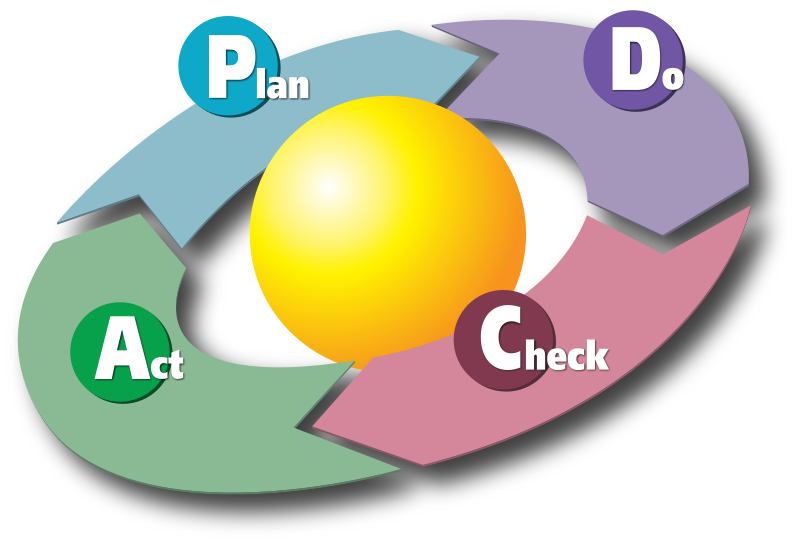
\includegraphics[width=0.60\textwidth]{img/pdca.png}
\caption{Ciclo PDCA}
\label{fig:PDCA}
\end{center}
\end{figure}

La qualit\`{a} dovr\`{a} rigurdare quindi, in primis, l\textquoteright{}organizzazione del lavoro al fine che esso sia il pi\`{u} possibile regolato e ordinato, poi potr\`{a} anche riflettersi nel progetto.

\paragraph*{Qualit\`{a} software}

Gli obiettivi di qualit\`{a} andranno distinti in ogni fase del ciclo di vita del software. Qui verranno elencati i principali obiettivi nelle fasi critiche, cio\`{e} le milestones del progetto.

\subparagraph{Analisi}
\begin{itemize}
\item Fissare incontri con i possibili clienti interrogandoli sulle funzionalit\`{a} desiderabili del prodotto;
\item Raccogliere pi\`{u} feed-back possibile, quindi tenere aggiornati i requisiti al fine di fornire un prodotto, il pi\`{u} possibile secondo le aspettative dei clienti.
\end{itemize}
\subparagraph{Progettazione}
\begin{itemize}
\item L\textquoteright{}architettura dovr\`{a}, ove possibile, integrare compenenti gi\`{a} realizzate e testate al fine di riutilizzarle senza realizzarle poi da zero;
\item L\textquoteright{}architettura dovr\`{a} implementare solo design patterns conosciuti e dimostati;
\item L\textquoteright{}architettura dovr\`{a} limitare il numero di dipendenze tra le componenti ed evitare le dipendenze cicliche;
\item L\textquoteright{}architettura dovr\`{a} utilizzare componenti che prevedono l\textquoteright{}utilizzo di classi che implementano metodi il cui codice non superi le 50 righe;
\item L\textquoteright{}architettura dovr\`{a} essere sottoposta a revisione da parte di entit\`{a} non direttamente coinvolte.
\end{itemize}
\subparagraph{Sviluppo}
\begin{itemize}
\item Il codice dell\textquoteright{}applicativo dovr\`{a} essere commentato nei punti critici;
\item Il codice dell\textquoteright{}applicativo dovr\`{a} avere una bassa complessit\`{a} ciclomatica\footnote{numero di casi di prova da effettuare nella fase di verifica del codice};
\item La compilazione del codice non dovr\`{a} fornire né errori né warnings\footnote{avvisi che indicano che parte di codice non viene utilizzato o pu\`{o} essere soggetto a errore a run time}.
\end{itemize}